\subsection{实践任务二：阻塞}
任务一用的 \texttt{func\_lab3} 在相关指令之间插入了 4 条 \texttt{addu \$0,\$0,\$0}，消费者落到写回之后才进入译码级，看不出写后读。
\texttt{func\_lab4} 把 \texttt{NOP} 宏改成空，\texttt{LI} 里只留下 3 条 \texttt{nop}。把 \texttt{inst\_ram} 换成
\texttt{soft/func\_lab4/obj/inst\_ram.coe}，用 \texttt{cpu132\_gettrace} 重新生成 \texttt{golden\_trace.txt}。
参考轨迹在 1.184\,ms 结束。

\subsubsection{未加阻塞时的写后读}
寄存器堆在写回级的时钟沿写入，译码级组合读出。生产者还在 EX、MEM 或 WB 时，译码级读到的是旧值；若该寄存器从未写过，仿真里就是 X。
\texttt{start.S} 里 \texttt{lui \$s0, 0} 之后只有 \texttt{jal n1\_lui\_test} 和延迟槽，测试入口第一条就是 \texttt{addiu \$s0, \$s0, 1}。
当这条 \texttt{addiu} 停在 ID 时，\texttt{lui \$s0} 正好在 WB，同拍读到 X。

\begin{verbatim}
[2537 ns] Error!!!
reference: PC = 0xbfc408b0, wb_rf_wnum = 0x10, wb_rf_wdata = 0x00000001
mycpu    : PC = 0xbfc408b0, wb_rf_wnum = 0x10, wb_rf_wdata = 0xxxxxxxxx
\end{verbatim}

\begin{figure}[H]
  \centering
  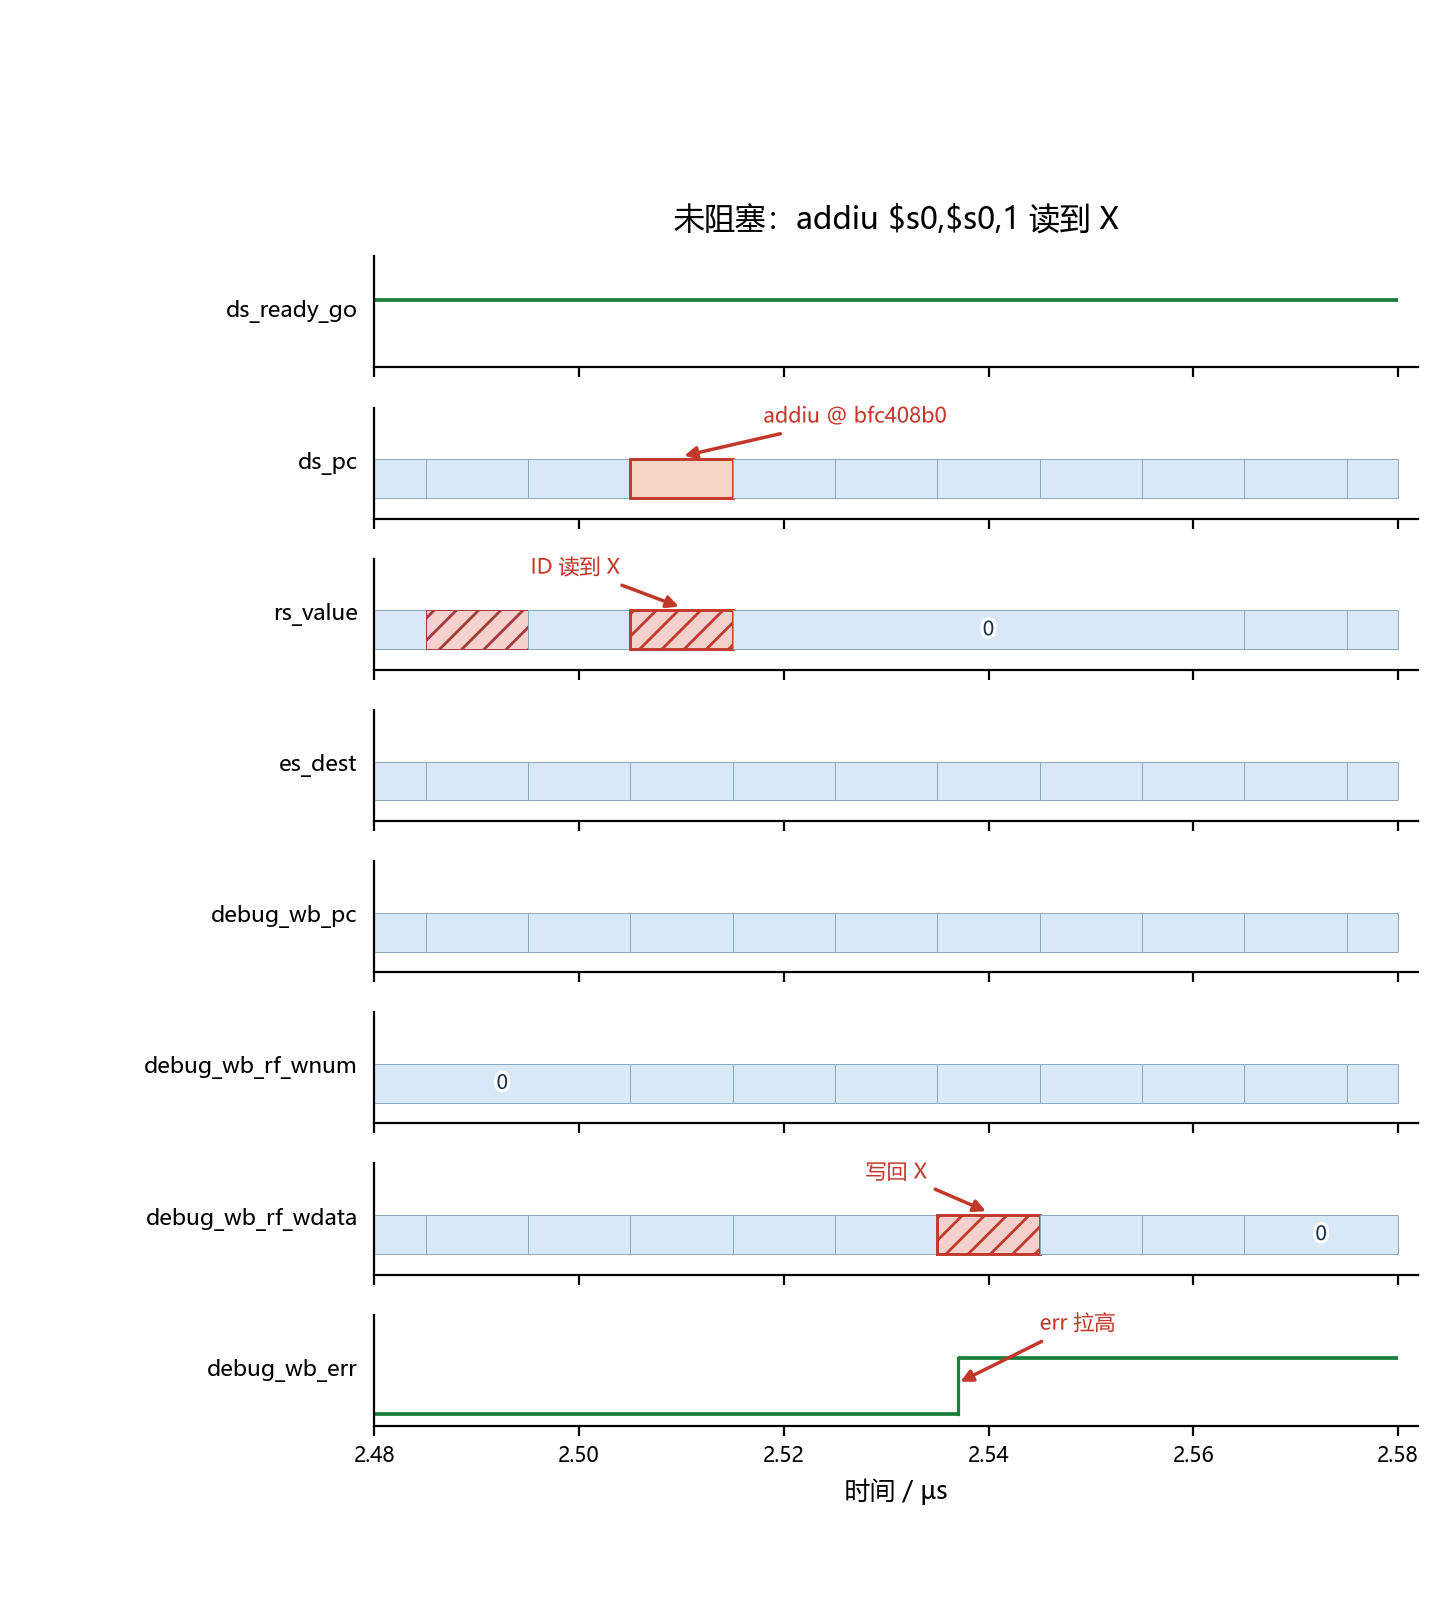
\includegraphics[width=\linewidth]{fig/stall_before.png}
  \caption{未阻塞。\texttt{ds\_pc=bfc408b0} 的 \texttt{addiu \$s0,\$s0,1} 在 ID 时 \texttt{rs\_value} 为 X，
  随后写回 X，\texttt{debug\_wb\_err} 拉高。}
\end{figure}

\subsubsection{阻塞逻辑}
译码级根据本条是否使用 \texttt{rs}/\texttt{rt}，与 EX、MEM、WB 的写目的比较。命中且目的不是 \texttt{\$0} 时，
\texttt{ds\_ready\_go=0}：IF 因 \texttt{ds\_allowin} 为低而停住，进入 EX 的 \texttt{valid} 为低，形成气泡。
写回与译码同拍时寄存器堆仍是旧值，因此 WB 命中也停一拍，下一拍再读。阻塞期间把 \texttt{br\_taken} 拉低，避免用旧比较结果改 PC。

\begin{verbatim}
assign ds_ready_go = ~(es_raw | ms_raw | ws_raw);
assign br_taken    = (...分支条件...) && ds_valid && ds_ready_go;
\end{verbatim}

EX、MEM 的 \texttt{valid}、\texttt{gr\_we}、\texttt{dest} 送到 ID；WB 用已有的 \texttt{ws\_to\_rf\_bus} 里的 \texttt{rf\_we}/\texttt{rf\_waddr}。

\begin{figure}[H]
  \centering
  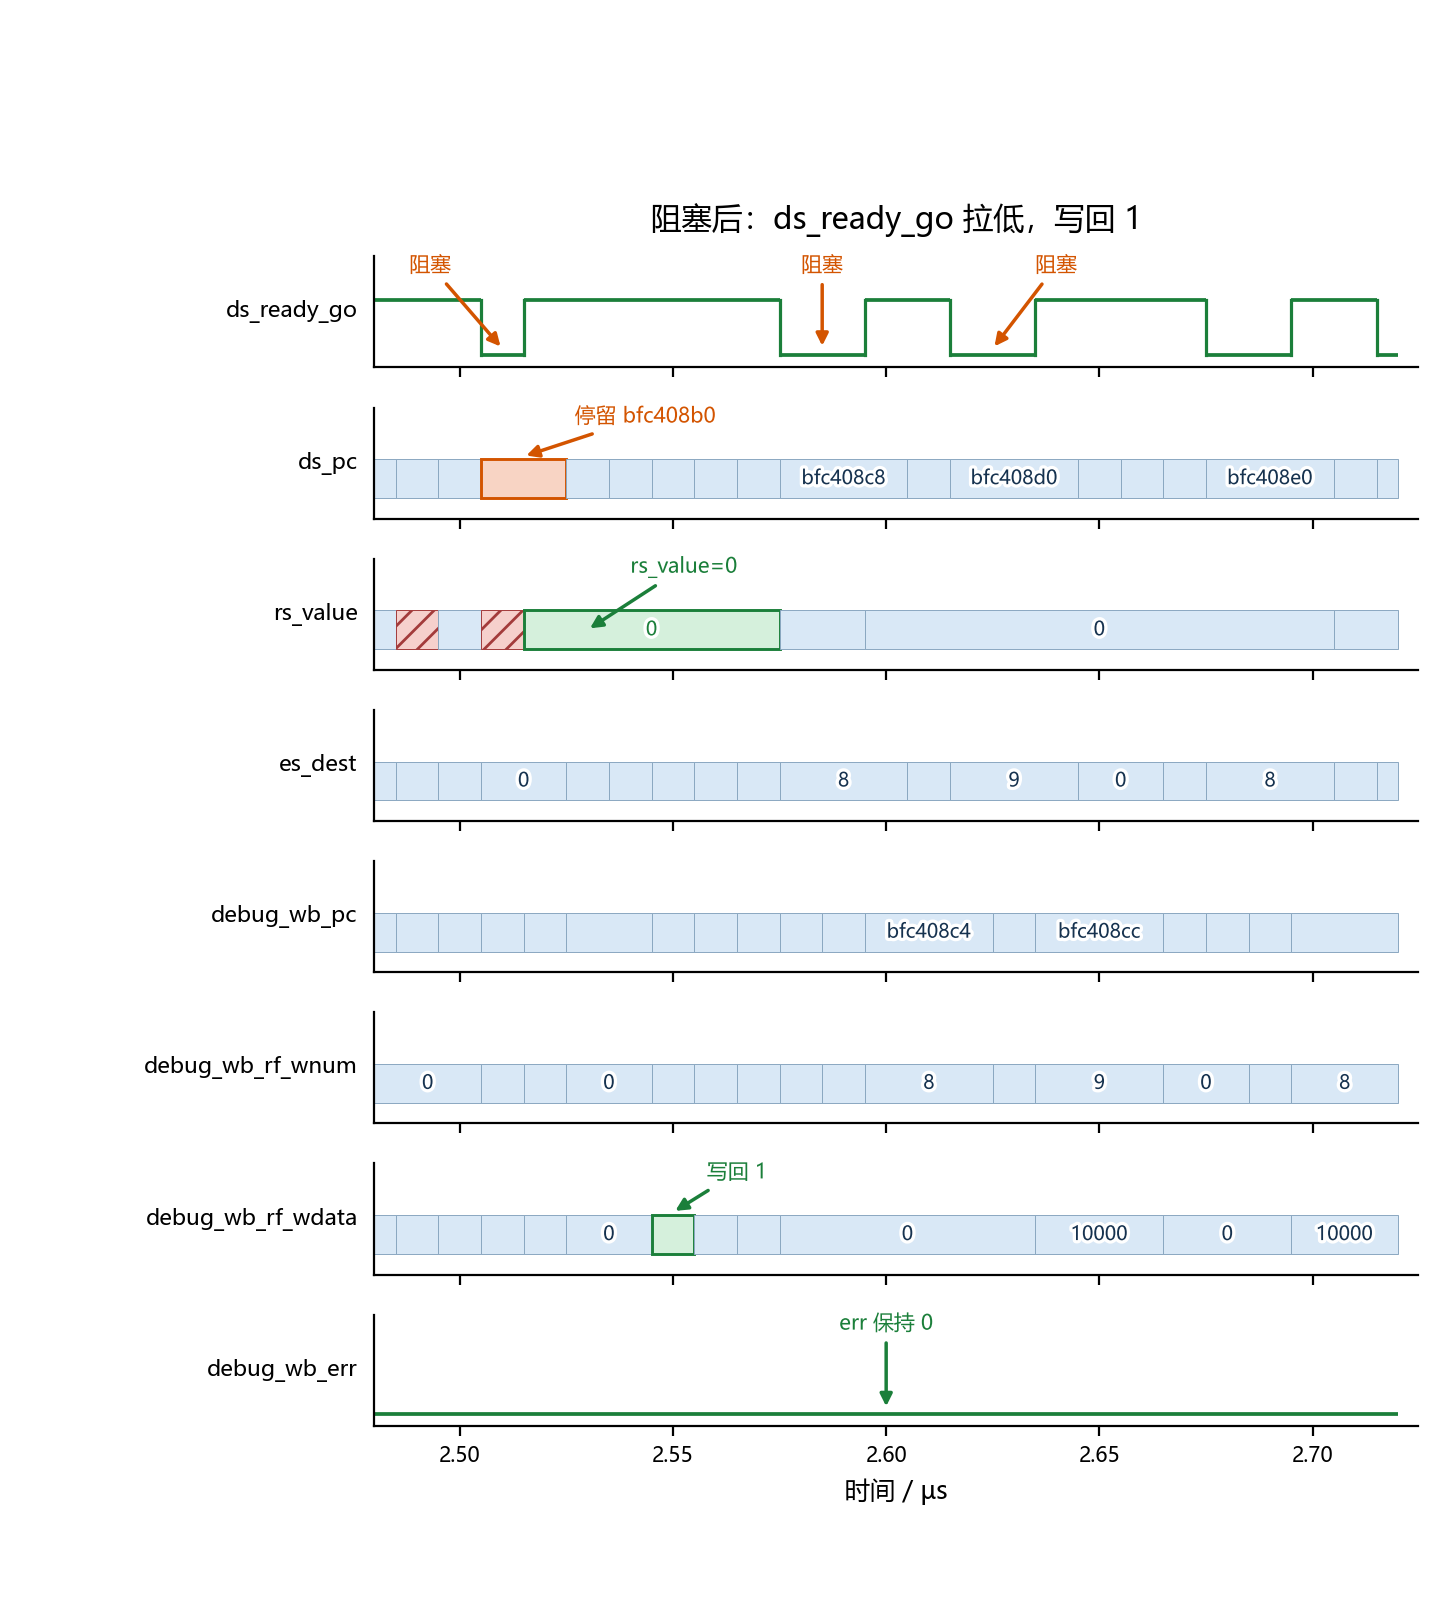
\includegraphics[width=\linewidth]{fig/stall_after.png}
  \caption{阻塞后同一段。\texttt{ds\_ready\_go} 多次拉低，\texttt{ds\_pc} 在 \texttt{bfc408b0} 停留，
  \texttt{rs\_value} 变为 0 后再放行。\texttt{debug\_wb\_err} 保持 0。}
\end{figure}

加阻塞后 23 个功能点全部通过，测试在 1.311\,ms 结束，比参考 CPU 的 1.184\,ms 多出约 $1.27\times10^{4}$ 个时钟（周期 10\,ns）。多出来的就是气泡。控制台末尾：
\begin{verbatim}
----[1310005 ns] Number 8'd23 Functional Test Point PASS!!!
Test end!
----PASS!!!
$finish called at time : 1310945 ns
\end{verbatim}

